\begin{frame}{Motivation}
  \begin{itemize}
    \item<1-> Histopathological analysis is central for cancer diagnosis.
    \item<2-> Manual image analysis is time-consuming and depends on expert judgement.
    \item<3-> In medical classification, false negatives for cancer-related tissue are especially costly.
    \item<4-> The goal is therefore recall-oriented improvement, not only higher accuracy.
  \end{itemize}
  \begin{block}<5->{Project Question}
    Can targeted binary expert classifiers correct the main weaknesses of a general PathMNIST classifier?
  \end{block}
\end{frame}

\begin{frame}{PathMNIST Dataset}
  \begin{columns}[T,onlytextwidth]
    \begin{column}{0.44\textwidth}
      \begin{itemize}
        \item 107,180 colorectal cancer histology patches.
        \item Splits: 89,996 train, 10,004 validation, 7,180 test.
        \item Nine tissue classes.
        \item Images available at $28 \times 28$ and $224 \times 224$ pixels.
      \end{itemize}
      \begin{block}{Cancer-related classes}
        Cancer-associated stroma and colorectal adenocarcinoma epithelium.
      \end{block}
    \end{column}
    \begin{column}{0.54\textwidth}
      \centering
      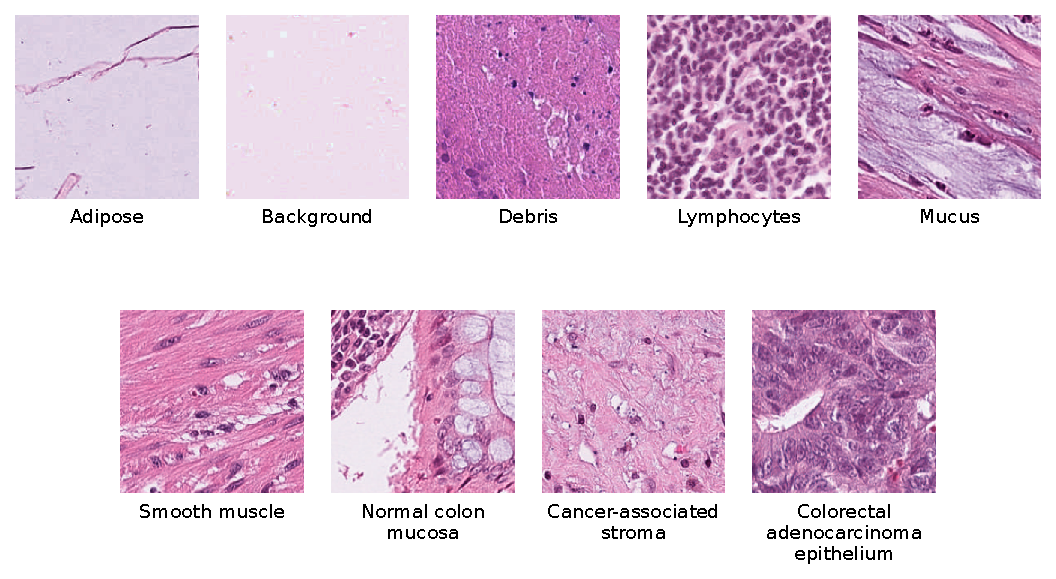
\includegraphics[width=\textwidth]{figures/pathmnist_class_examples}
    \end{column}
  \end{columns}
\end{frame}

\begin{frame}{Class Distribution}
  \centering
  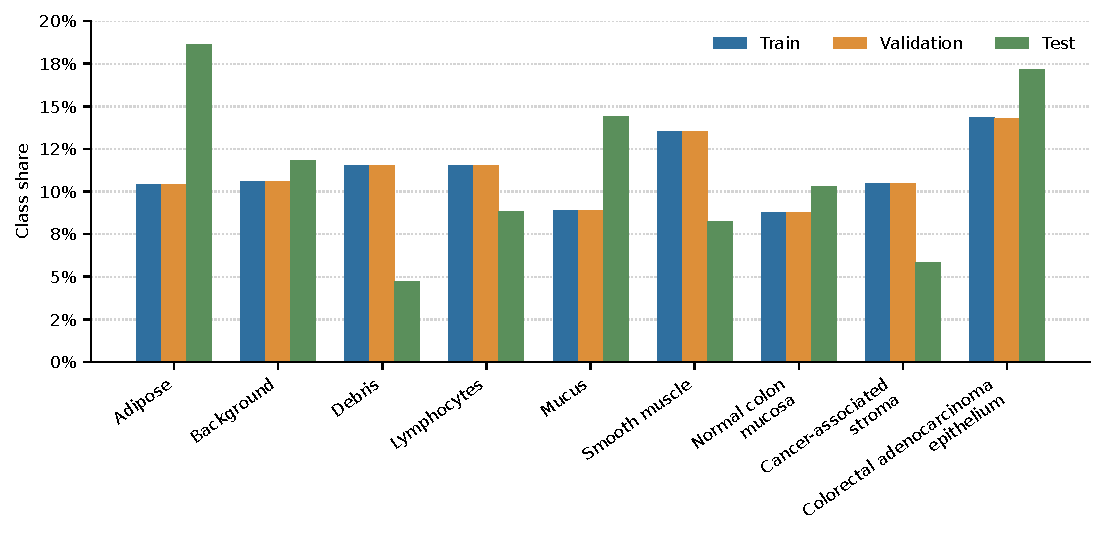
\includegraphics[width=0.82\textwidth]{figures/pathmnist_class_distribution}
  \vspace{0.4em}
  \begin{itemize}
    \item Smooth muscle and epithelium are among the largest class fractions.
    \item Stroma is clinically relevant but harder for the baseline model.
  \end{itemize}
\end{frame}

\section{Model Development}
